\documentclass{article}
\usepackage[utf8]{inputenc}
\usepackage[spanish,mexico]{babel}
\usepackage[margin=2.5cm]{geometry}
\usepackage{graphicx}
\usepackage[export]{adjustbox}
\usepackage{caption}
\usepackage{subcaption}
\usepackage{fancyhdr}
\usepackage{avant}
\usepackage[T1]{fontenc}
\usepackage{pdfpages}
\pagestyle{fancy}
\fancyhf{}
\renewcommand*\familydefault{\sfdefault}

\title{Proyecto Seguridad Informatica}
\author{Gonzalez Calzada Maximiliano}
\date{\today}

\begin{document}

    \thispagestyle{empty}
        
    \begin{figure}[ht]
        \minipage{0.16\textwidth}
            
\includegraphics[width=2.2cm]{IPN_Logo.pdf}
            \label{LogoIPN}
        \endminipage
        \hspace{0.60\textwidth}
        \minipage{0.22\textwidth}
            
\includegraphics[width=3cm]{UPIICSA_Logo.pdf}
            \label{LogoUPIICSA}
        \endminipage
    \end{figure}
	
	\begin{center}
        \vspace{0.8cm}
        \LARGE
        \textbf{INSTITUTO POLITÉCNICO NACIONAL}
        
        \vspace{0.8cm}
        \LARGE
        \textbf{UNIDAD PROFESIONAL INTERDISCIPLINARIA DE INGENIERÍA Y CIENCIAS SOCIALES Y ADMINISTRATIVAS}
        
        \vspace{0.8cm}	
        \Large
        \textbf{SEGURIDAD INFORMÁTICA}

        \vspace{0.8cm}
        \LARGE
        \textbf{"Web API Security Scanner"}

    \end{center}

        \vspace{0.6cm}
        \large	
        \textbf{Equipo 2} \\
        \normalsize
        INTEGRANTES \\
        \vspace{0.2cm}
        \normalsize
        \begin{itemize}
            \item \textbf{Gonzalez Calzada Maximiliano}
            \item \textbf{Hernandez Garcia Juan Jose}
            \item \textbf{Maldonado Martínez Kevin Noel}
            \item \textbf{Martínez Lagunas Andrik Jeovany}
            \item \textbf{Muñoz Castro Angel Daniel}
        \end{itemize}
        
        \vspace{0.8cm}
        \normalsize	
        DOCENTE \\
        \vspace{0.2cm}
        \large
        \textbf{Julia Alicia Ortega Avalos}

        \vspace{1cm}
        
        \vspace{1cm}
        \large
        \rightline{\textbf{4NM42} - \textbf{Diciembre 2024}}
	
	\newpage
    
    \section{Objetivo}

    Desarrollar una herramienta que escanee las API web en busca de vulnerabilidades de seguridad, asegurando que sean sólidas contra amenazas comunes y proporcionando recomendaciones de mejora. Puede ayudar a demostrar el cumplimiento de es- tas normativas. La herramienta no solo identificará vulnerabilidades ya existentes, sino que también puede servir como un medio proactivo para detectar configuraciones inseguras y prácticas deficientes en la implementación de APIs.

    \section{Alcance}

    \subsection{Cobertura de Seguridad:}
    \begin{itemize}
        \item \textbf{Autenticación y Autorización}: Revisar las configuraciones de autenticación (JWT, OAuth) y control de acceso.
        \item \textbf{Validación de Entrada}: Identificar vulnerabilidades de inyección (SQL, XSS, comandos).
        \item \textbf{Limitación de Tarifas y Exposición de Datos Sensibles}: Comprobar la limitación de tasa para evitar abusos y verificar si se transmiten datos sensibles sin cifrado.
        \item \textbf{Detección de Amenazas Comunes}: Enfocarse en las vulnerabilidades descritas en el OWASP API Security Top Ten.
    \end{itemize}

    \subsection{Límites del Proyecto:}
    \begin{itemize}
        \item \textbf{Exclusiones}: La herramienta no se enfocará en realizar pruebas de rendimiento o funcionalidad de la API; su único enfoque será la seguridad.
        \item \textbf{Limitaciones Técnicas}: El alcance inicial del proyecto no incluirá integración avanzada con sistemas de terceros para generación de reportes o monitoreo, aunque esta funcionalidad podría considerarse en versiones futuras.
    \end{itemize}

    \section{Justificación}

    En México, el panorama de ciberseguridad ha mostrado un aumento significativo en los incidentes relacionados con APIs web. Casos recientes han expuesto vulnerabilidades críticas, como el hackeo a sistemas gubernamentales que resultó en la filtración de datos sensibles en 2022, y los ataques al sector financiero reportados por la Comisión Nacional Bancaria y de Valores (CNBV) en 2023, donde APIs bancarias fueron explotadas para realizar fraudes y acceder a información confidencial. Estos incidentes resaltan la urgente necesidad de fortalecer la seguridad en APIs, especialmente en un contexto donde los cibercriminales emplean tácticas cada vez más sofisticadas para identificar y aprovechar puntos débiles.

    En la actualidad, las API son fundamentales para el funcionamiento de aplicaciones modernas, permitiendo la comunicación entre diferentes sistemas y servicios. Con el aumento de su uso, también ha crecido la superficie de ataque, haciendo que la seguridad de las API sea una prioridad. A continuación se detallan las razones que apoyan la necesidad de un escáner de seguridad para APIs web:

    \begin{itemize}
        \item \textbf{Creciente Dependencia de APIs}: Con la propagación de arquitecturas basadas en microservicios y el uso extensivo de servicios web, las APIs se han convertido en un punto de entrada crucial para las aplicaciones. Esto las convierte en un objetivo atractivo para los atacantes.
        \item \textbf{Vulnerabilidades Comunes}: Existen vulnerabilidades comunes en las APIs, como las descritas en el OWASP API Security Top Ten. Un escáner automatizado puede ayudar a identificar y mitigar estas vulnerabilidades antes de que sean explotadas.
        \item \textbf{Automatización y Eficiencia}: Realizar análisis de seguridad manualmente es intensivo en tiempo y recursos. Una herramienta automatizada permite escanear múltiples APIs de forma eficiente, liberando a los equipos de seguridad para que se concentren en análisis más profundos y en la remediación de problemas detectados.
        \item \textbf{Mejora Continua en la Seguridad}: La generación de informes detallados con recomendaciones proporciona a los desarrolladores y equipos de seguridad una guía para mejorar continuamente la postura de seguridad de sus APIs.
        \item \textbf{Educación y Conciencia}: Incluir una interfaz amigable y documentación clara no solo hace que la herramienta sea accesible, sino que también educa a los usuarios sobre las prácticas de seguridad y la importancia de proteger sus APIs.
        \item \textbf{Cumplimiento Normativo}: Muchas organizaciones están sujetas a regulaciones que exigen la implementación de prácticas de seguridad adecuadas. Un escáner de seguridad puede ayudar a demostrar el cumplimiento de estas normativas.
        \item \textbf{Proactividad ante Amenazas}: La herramienta no solo identificará vulnerabilidades ya existentes, sino que también puede servir como un medio proactivo para detectar configuraciones inseguras y prácticas deficientes en la implementación de APIs. Adoptar un enfoque proactivo en la seguridad permite que las empresas se anticipen a posibles ataques y mantengan su infraestructura más segura.
    \end{itemize}

    \section{Marco teórico}

    \subsection{Definición de Seguridad}
    La seguridad se refiere al conjunto de medidas, procesos y prácticas diseñadas para proteger recursos valiosos frente a posibles riesgos, amenazas o accesos no autorizados. En un sentido amplio, abarca la protección de bienes tangibles e intangibles, asegurando su disponibilidad, integridad y confidencialidad.

    \subsection{Seguridad Informática}
    La seguridad informática se centra en la protección de sistemas de información, redes y datos frente a amenazas que puedan comprometer su confidencialidad, integridad o disponibilidad. Esto incluye la implementación de controles técnicos, como cifrado y firewalls, y procesos administrativos para prevenir accesos no autorizados y minimizar el impacto de posibles ataques. La seguridad informática es crucial en un mundo donde los datos digitales son un recurso estratégico tanto para individuos como para organizaciones.

    \subsection{Seguridad en la Red}
    La seguridad en la red engloba las políticas, tecnologías y prácticas utilizadas para proteger la infraestructura de redes y los datos que se transfieren a través de ellas. Esto incluye prevenir ataques como interceptación de datos (sniffing), denegación de servicio (DoS), intrusiones y malware. Las medidas comunes en la seguridad de red incluyen el uso de firewalls, sistemas de detección y prevención de intrusiones (IDS/IPS) y protocolos de cifrado como TLS/SSL.

    \subsection{Seguridad en la Nube}
    La seguridad en la nube es el conjunto de políticas, tecnologías y controles diseñados para proteger datos, aplicaciones y servicios alojados en plataformas de computación en la nube. Incluye aspectos como la protección de datos en reposo y en tránsito, el cumplimiento de normativas, y la gestión de accesos y permisos en entornos compartidos. La adopción masiva de servicios en la nube ha aumentado los riesgos, haciendo esencial la implementación de medidas robustas como el cifrado, autenticación multifactor y auditorías regulares.

    \subsection{Introducción a las APIs Web}
    \subsubsection{Definición}
    Las APIs (Interfaz de Programación de Aplicaciones) permiten que diferentes aplicaciones se comuniquen entre sí. Son cruciales en la arquitectura de software moderna, especialmente en aplicaciones web y móviles. Son mecanismos que permiten que diferentes aplicaciones y sistemas intercambien datos y funciones entre sí. Son esenciales en el entorno digital actual, especialmente en aplicaciones web y móviles, donde facilitan la interoperabilidad y la integración de diversas funcionalidades. Las APIs son la columna vertebral de arquitecturas modernas como los microservicios, permitiendo que distintos componentes de software se comuniquen y trabajen juntos sin estar directamente acoplados.

    \subsubsection{Importancia}
    Facilitan la integración y la interoperabilidad, pero también presentan riesgos de seguridad que deben ser gestionados adecuadamente. La popularidad de las APIs ha crecido junto con el uso de servicios en la nube, lo que ha incrementado su papel en las estrategias de negocio de las organizaciones. Sin embargo, esta integración trae consigo importantes riesgos de seguridad, ya que las APIs se exponen frecuentemente a redes públicas, convirtiéndolas en un blanco atractivo para atacantes. Una API sin las medidas de seguridad adecuadas puede ser la puerta de entrada para amenazas que afecten la integridad, confidencialidad y disponibilidad de los sistemas empresariales. La seguridad en las APIs implica implementar mecanismos de autenticación, autorización, validación de datos y monitoreo constante para mitigar estos riesgos.

    \subsection{La Seguridad Informática Relacionados con las APIs}
    En el contexto de seguridad informática, existen varios subtemas clave que se aplican específicamente a la seguridad de APIs:

    \begin{itemize}
        \item \textbf{Autenticación y Autorización}: La autenticación asegura que solo usuarios válidos accedan a una API, mientras que la autorización define los permisos y el nivel de acceso que cada usuario posee. Los estándares como OAuth 2.0 y JWT (JSON Web Tokens) son ampliamente utilizados en la autenticación de APIs para proporcionar acceso controlado y seguro.
        \item \textbf{Integridad de Datos}: Este principio garantiza que la información transmitida a través de la API no sea alterada durante el tránsito. La integridad de datos puede asegurarse mediante el uso de protocolos como HTTPS y el cifrado de datos sensibles, evitando ataques que alteren la información durante su transmisión.
        \item \textbf{Monitoreo y Registro}: Es fundamental registrar y monitorear las actividades dentro de una API para detectar comportamientos anómalos que puedan ser indicativos de intentos de ataque. Herramientas como los sistemas de detección de intrusiones (IDS) pueden integrarse para alertar sobre accesos inusuales o patrones de solicitudes sospechosas.
    \end{itemize}

    \subsection{Amenazas Comunes a las APIs}
    \begin{itemize}
        \item \textbf{Inyección SQL}: Permite a los atacantes ejecutar consultas maliciosas en la base de datos.
        \item \textbf{XSS}: Aprovecha la confianza del navegador en las API para ejecutar código en el contexto de un usuario.
        \item \textbf{Falsificación de solicitudes entre sitios (CSRF)}: Permite a un atacante hacer solicitudes en nombre de un usuario autenticado.
        \item \textbf{Desbordamiento de datos}: Implica enviar un volumen alto de datos a la API con el objetivo de desestabilizar o hacerla inaccesible.
    \end{itemize}

    \subsection{OWASP y la Seguridad en APIs}
    El Open Web Application Security Project (OWASP) ha publicado una lista de los diez riesgos principales para la seguridad de APIs, conocida como OWASP API Security Top Ten. Este listado destaca vulnerabilidades comunes como la autenticación rota, la exposición excesiva de datos y la falta de limitación de tasas. La guía OWASP es una referencia fundamental en el desarrollo seguro de APIs, ya que proporciona recomendaciones prácticas para abordar las amenazas de seguridad más relevantes en entornos de API.

    \subsection{La Seguridad en APIs en el Contexto Empresarial}
    Las empresas de sectores como finanzas, salud y comercio electrónico dependen cada vez más de las APIs para optimizar operaciones, gestionar datos y facilitar la integración con terceros. Sin embargo, según un informe de Akamai, el 78\% de las organizaciones han experimentado incidentes de seguridad relacionados con APIs en el último año. Además, las vulnerabilidades en APIs pueden ocasionar pérdidas anuales de hasta 87 mil millones de dólares, según Businesswire. Por lo tanto, asegurar estas interfaces se convierte en una prioridad no solo para proteger los activos digitales y la información confidencial, sino también para cumplir con normativas y regulaciones de seguridad.

    \subsection{Estrategias de seguridad para las APIs}
    Implementar estrategias de seguridad en APIs implica un enfoque multidimensional que incluye las siguientes prácticas:

    \begin{itemize}
        \item \textbf{Autenticación y Autorización Fortalecidas}: Usar autenticación multifactor y revisar permisos con regularidad.
        \item \textbf{Limitación de Tasas (Rate Limiting)}: Restringir el número de solicitudes permitidas en un tiempo determinado para evitar ataques de denegación de servicio (DoS).
        \item \textbf{Validación de Datos y Filtrado de Entradas}: Validar los datos que ingresan a la API para evitar inyecciones maliciosas.
        \item \textbf{Cifrado de Comunicación}: Usar HTTPS para garantizar que los datos en tránsito estén protegidos contra interceptaciones.
    \end{itemize}

    \newpage
    \section{Planteamiento de la solución}

    \begin{itemize}
        \item \textbf{Identificación de Amenazas Comunes en APIs}: Revise el OWASP API Security Top Ten y otras normativas de seguridad para reconocer las vulnerabilidades más frecuentes en APIs.
        \item \textbf{Selección de Herramientas y Lenguaje de Programación}: Escoja un lenguaje adecuado (por ejemplo, Python o JavaScript) y herramientas de escaneo de seguridad (como OWASP ZAP o Burp Suite) que se integren efectivamente para identificar y mitigar riesgos.
        \item \textbf{Desarrollo de Módulos de Seguridad}: Implemente módulos específicos para detectar vulnerabilidades, como autenticación, autorización, inyección de SQL, XSS, y otros. Cada módulo debe ser capaz de realizar pruebas automatizadas y reportar sus hallazgos.
        \item \textbf{Diseño de la Interfaz de Usuario}: Cree una interfaz intuitiva, ya sea web o en línea de comandos, que permita a los usuarios configurar las API a escanear, seleccionar parámetros y monitorear el progreso de los escaneos.
        \item \textbf{Implementación de Monitoreo y Alerta}: Configure un sistema de monitoreo y alertas en tiempo real para detectar actividad sospechosa y registrar logs detallados de cada interacción de la API.
        \item \textbf{Pruebas de Seguridad Automatizadas}: Realice pruebas automatizadas y pruebas de penetración en entornos controlados, usando datos simulados para verificar la capacidad de detección y respuesta ante ataques.
        \item \textbf{Documentación y Capacitación}: Desarrolle documentación clara y detallada sobre cómo usar la herramienta, interpretando resultados y aplicando recomendaciones de seguridad. Incluya guías prácticas para el equipo de desarrollo y personal de seguridad.
        \item \textbf{Mantenimiento y Actualización Continua}: Programe revisiones y actualizaciones regulares de la herramienta para garantizar que se mantenga al día con nuevas vulnerabilidades y mejoras de seguridad en APIs.        
    \end{itemize}
    \section{Diagrama de procesos}
    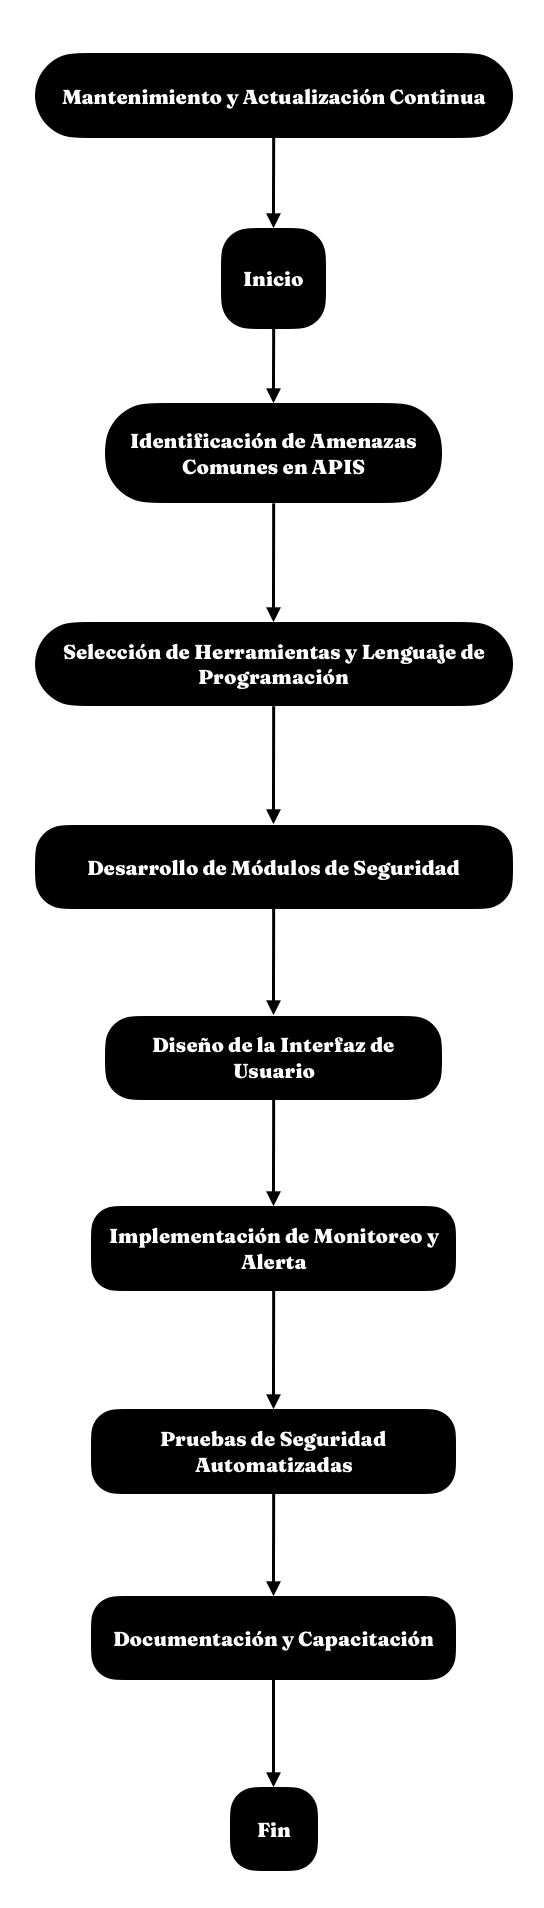
\includegraphics[height=1\textwidth, center]{Figura1.png}
    \section{Planeación}
    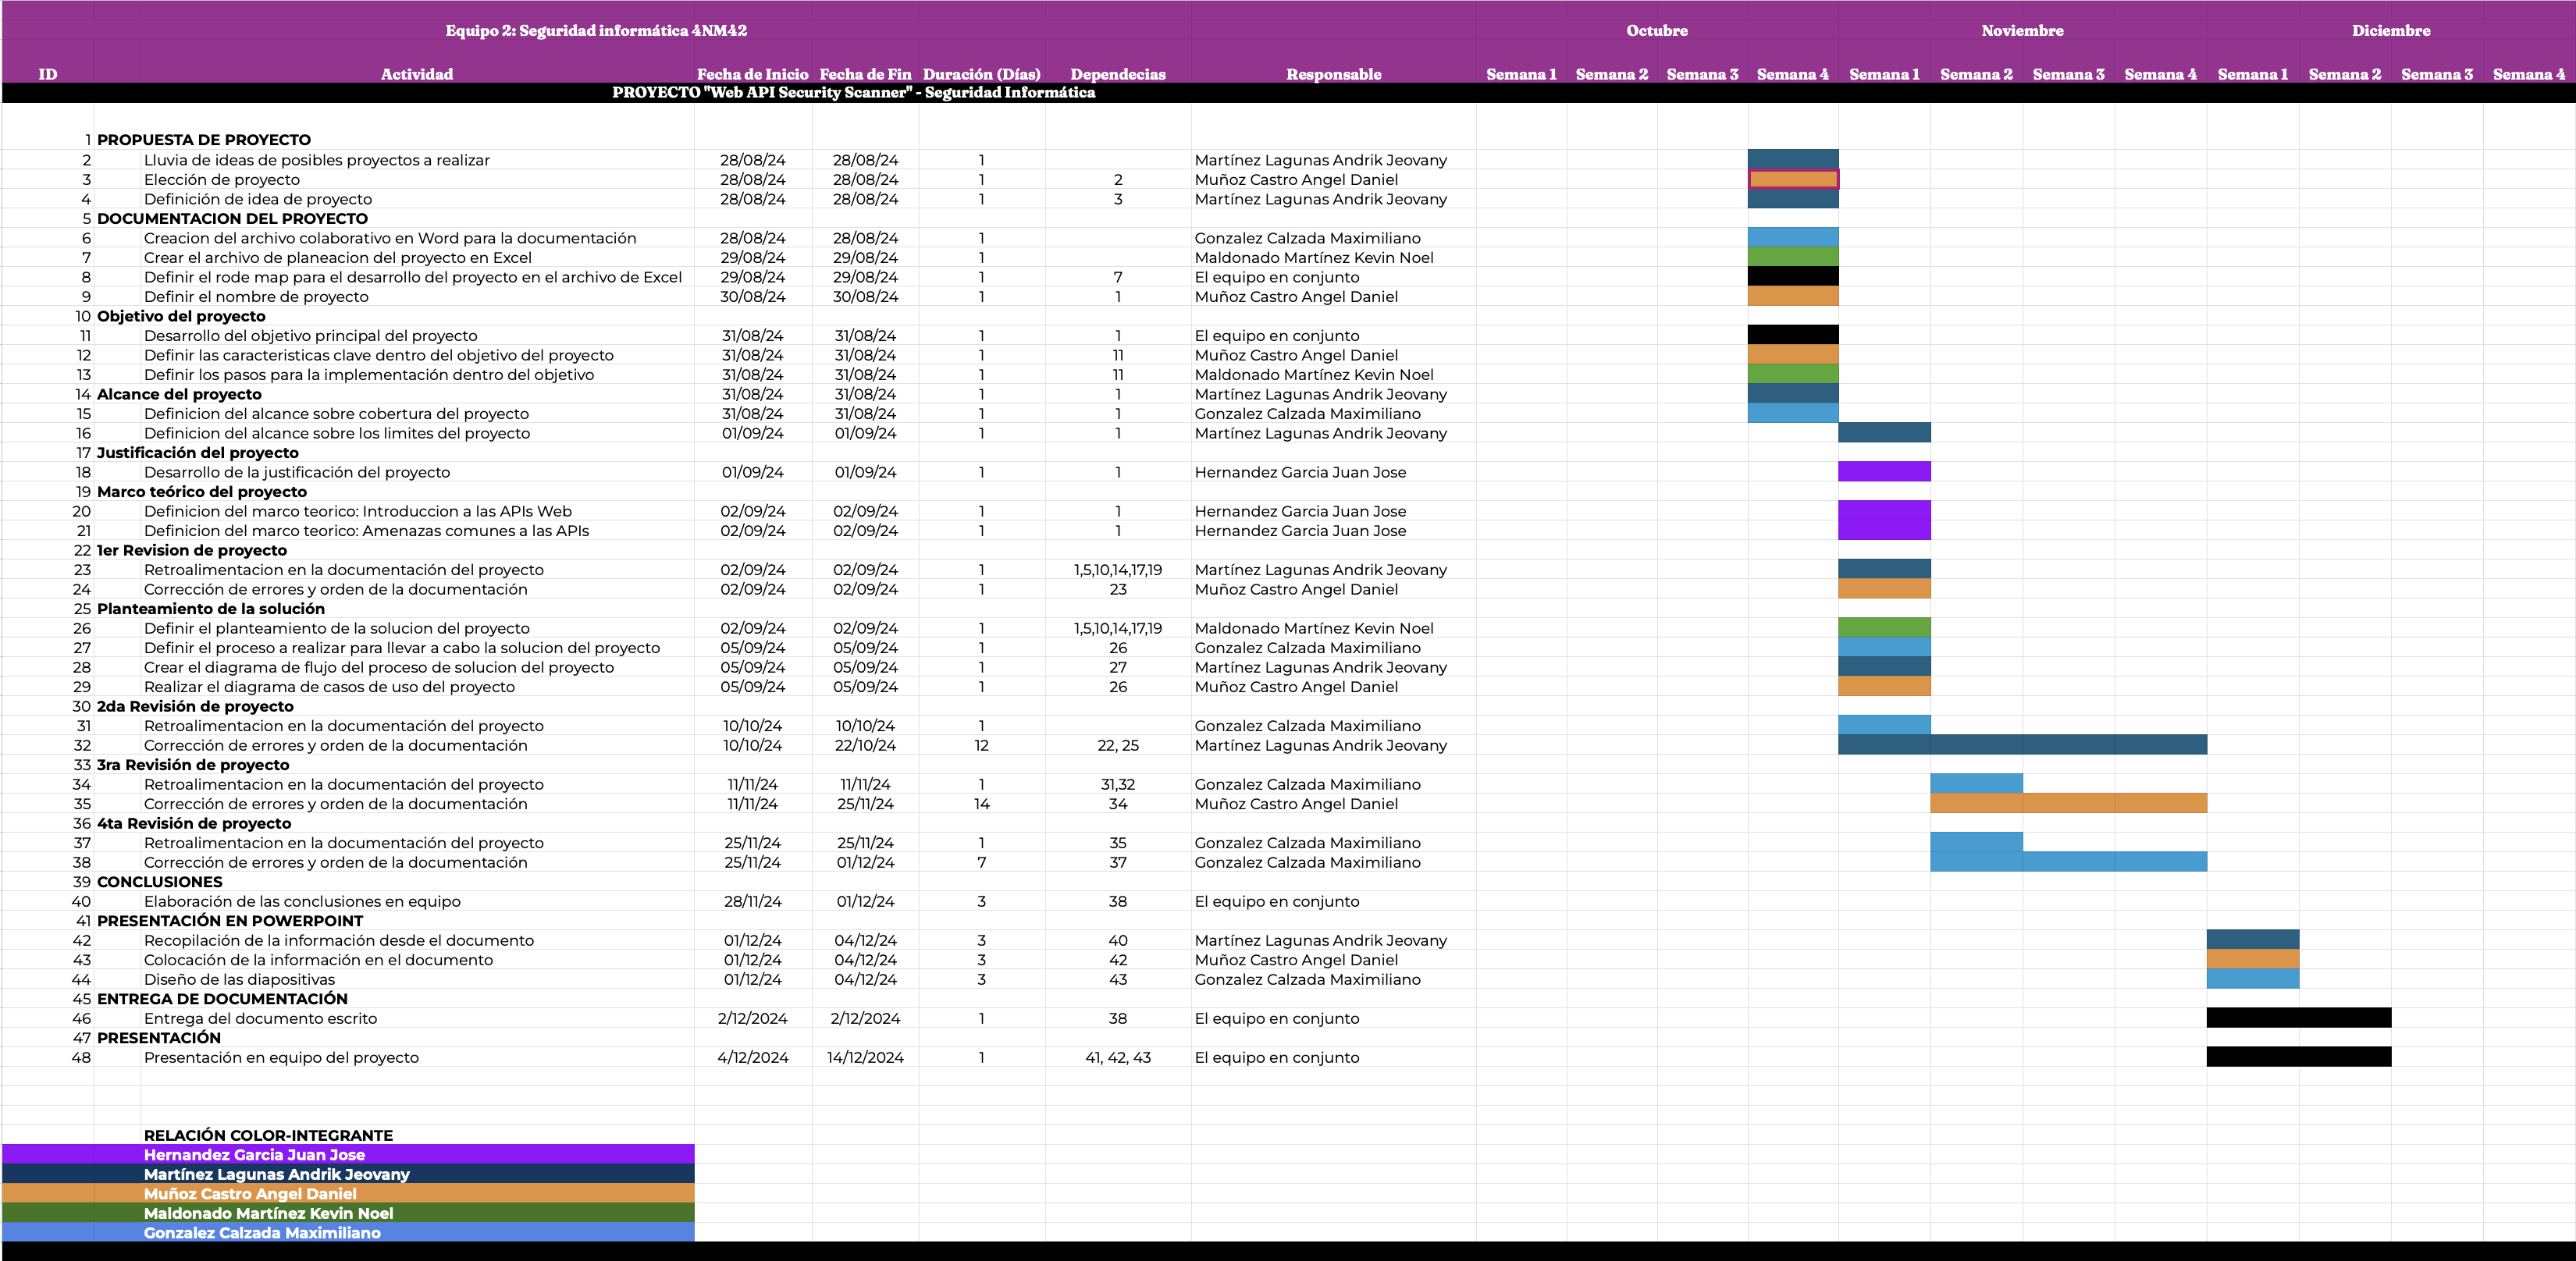
\includegraphics[width=0.8\textwidth, center]{Figura2.png}

    \section{Conclusiones}
    A lo largo del desarrollo del proyecto "Web API Security Scanner", se ha logrado identificar y abordar una problemática relevante en el ámbito de la seguridad informática: la protección de las interfaces de programación de aplicaciones (APIs). Estas conclusiones resumen las principales lecciones aprendidas, resultados obtenidos y los retos futuros derivados de este trabajo.
    \\[2\baselineskip]
    En primer lugar, el análisis realizado confirma la creciente dependencia de las APIs en los entornos empresariales modernos y los riesgos inherentes asociados a su uso. En este contexto, el desarrollo de herramientas específicas, como el escáner presentado, es esencial para fortalecer la seguridad de los sistemas que utilizan APIs, minimizando su exposición a amenazas comunes como inyecciones SQL, XSS y ataques de fuerza bruta. La integración de estándares como OWASP API Security Top Ten ha sido un factor clave para asegurar que la herramienta aborda vulnerabilidades críticas de manera efectiva.
    \\[2\baselineskip]
    Un aspecto destacado del proyecto es la implementación de prácticas de seguridad proactivas, que no solo buscan identificar fallos existentes, sino también prevenir configuraciones inseguras y fomentar una cultura de desarrollo seguro. Esto subraya la importancia de la seguridad como un componente integral y continuo en el ciclo de vida del desarrollo de software, en lugar de un paso final correctivo.
    \\[2\baselineskip]
    Además, la colaboración multidisciplinaria y el uso de tecnologías robustas como Python y OWASP ZAP han permitido construir una solución técnica sólida, capaz de automatizar procesos de análisis que tradicionalmente requerían una inversión significativa de tiempo y recursos. Este enfoque automatizado no solo mejora la eficiencia, sino que también proporciona a los equipos de desarrollo y seguridad un acceso más rápido a información crítica para la toma de decisiones.
    \\[2\baselineskip]
    Sin embargo, el proyecto también ha evidenciado desafíos importantes. Entre ellos, la dificultad para integrar sistemas de monitoreo en tiempo real y la necesidad de mantener actualizada la herramienta frente a nuevas amenazas y cambios en el panorama tecnológico. Asimismo, se identificó la importancia de la capacitación continua para garantizar que los usuarios finales comprendan y apliquen correctamente las recomendaciones proporcionadas por el escáner.
    \\[2\baselineskip]
    En conclusión, el "Web API Security Scanner" representa un paso significativo hacia el fortalecimiento de la seguridad en APIs, contribuyendo a la reducción de riesgos y al cumplimiento de normativas en un entorno cada vez más digitalizado. A futuro, la expansión de sus capacidades, incluyendo la integración con plataformas de monitoreo avanzadas y el soporte para un mayor número de lenguajes y frameworks, será esencial para mantener su relevancia y efectividad. Este proyecto no solo refuerza la seguridad técnica, sino que también fomenta un cambio de paradigma hacia un enfoque más consciente y preventivo en la gestión de riesgos digitales.

    \section{Demostración}
    \section{Referencias}

\end{document}

